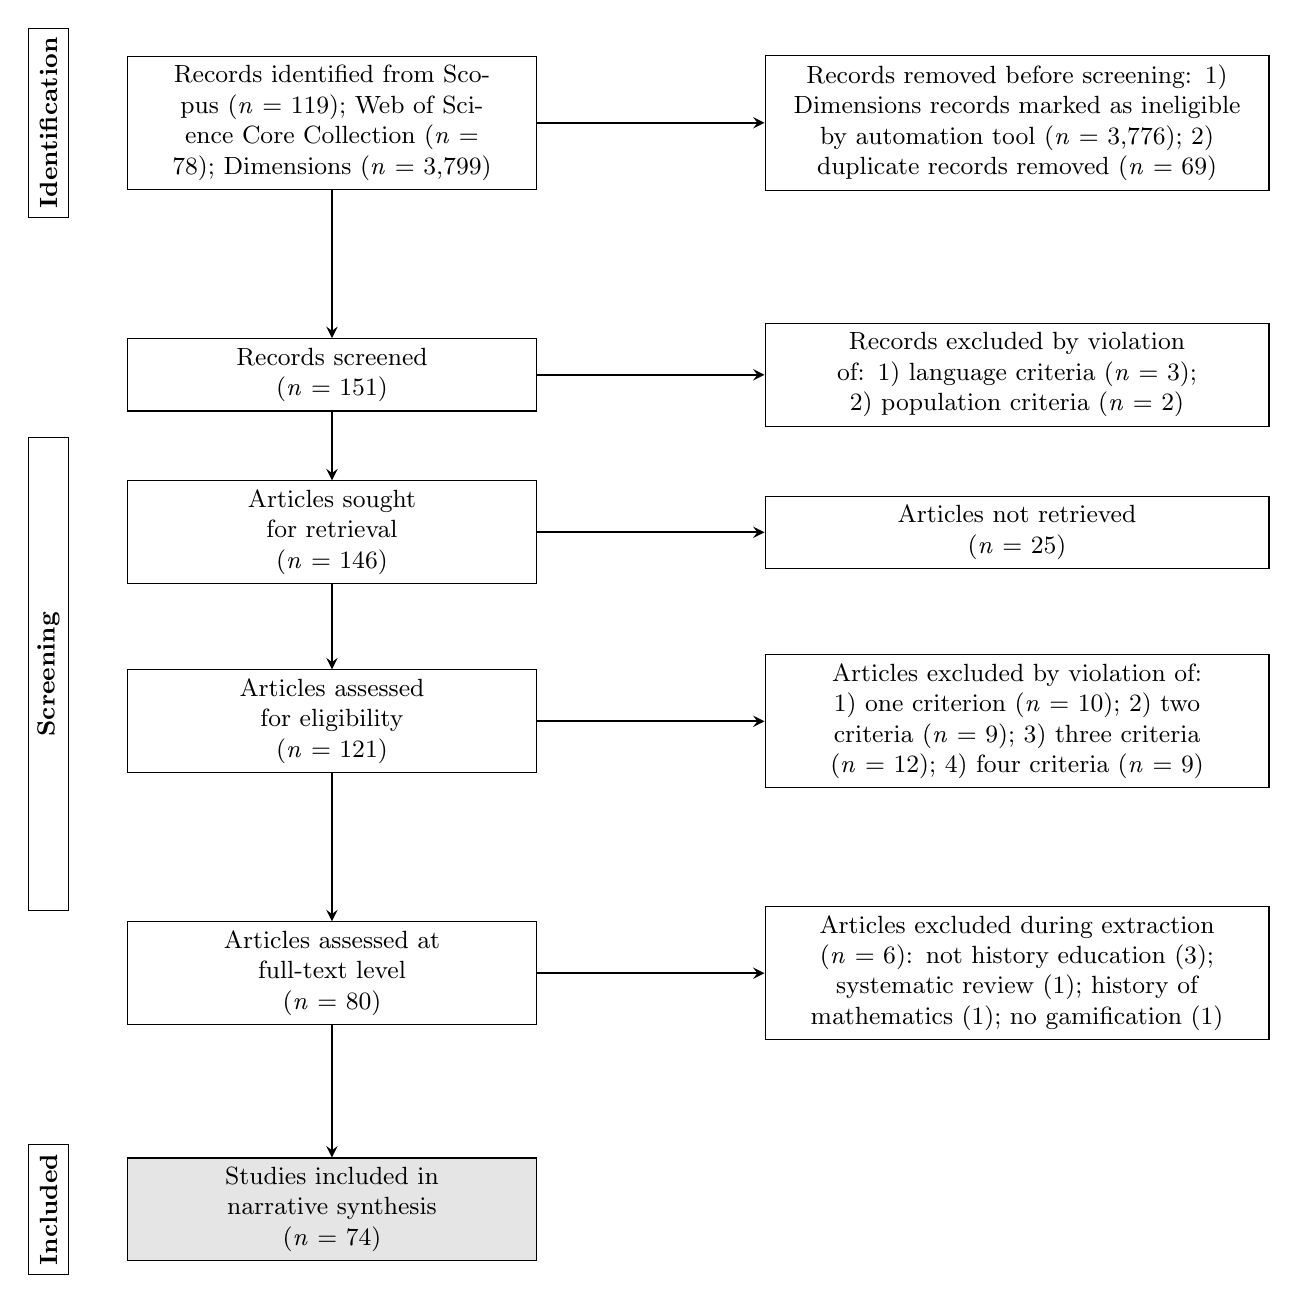
\begin{tikzpicture}[
  box/.style = {draw, align=center, font=\small},
  lbox/.style = {box, text width=48mm, minimum width=52mm},
  rbox/.style = {box, text width=60mm, minimum width=64mm},
  arrow/.style = {thick,-stealth}
]

% Natural \textwidth layout (17cm). No resizebox.
% Left column center x=2.8, right column center x=11.5
% Phase labels at x=-0.8

% Row 1: y=0
\node [lbox] (records) at (2.8,0)
  {Records identified from
   Scopus (\textit{n} = 119);
   Web of Science
   Core Collection (\textit{n} = 78);
   Dimensions (\textit{n} = 3,799)};

\node [rbox] (removed) at (11.5,0)
  {Records removed before screening:
   1) Dimensions records marked as ineligible
   by automation tool (\textit{n} = 3,776);
   2) duplicate records removed (\textit{n} = 69)};

% Row 2: y=-3.2
\node [lbox] (screened) at (2.8,-3.2)
  {Records screened\\(\textit{n} = 151)};

\node [rbox] (excluded) at (11.5,-3.2)
  {Records excluded by violation of:
   1) language criteria (\textit{n} = 3);
   2) population criteria (\textit{n} = 2)};

% Row 3: y=-5.2
\node [lbox] (sought) at (2.8,-5.2)
  {Articles sought\\for retrieval\\(\textit{n} = 146)};

\node [rbox] (notret) at (11.5,-5.2)
  {Articles not retrieved\\(\textit{n} = 25)};

% Row 4: y=-7.6
\node [lbox] (assessed) at (2.8,-7.6)
  {Articles assessed\\for eligibility\\(\textit{n} = 121)};

\node [rbox] (exclude) at (11.5,-7.6)
  {Articles excluded by violation of:
   1) one criterion (\textit{n} = 10);
   2) two criteria (\textit{n} = 9);
   3) three criteria (\textit{n} = 12);
   4) four criteria (\textit{n} = 9)};

% Row 5: y=-10.8 (gap for tall row 4 right box)
\node [lbox] (fulltext) at (2.8,-10.8)
  {Articles assessed at\\full-text level\\(\textit{n} = 80)};

\node [rbox] (excludefull) at (11.5,-10.8)
  {Articles excluded during extraction (\textit{n} = 6):
   not history education (3);
   systematic review (1);
   history of mathematics (1);
   no gamification (1)};

% Row 6: y=-13.8
\node [lbox, fill=gray!20] (included) at (2.8,-13.8)
  {Studies included in\\narrative synthesis\\(\textit{n} = 74)};

% Phase labels
\node [box, align=center, minimum height=2cm, minimum width=5mm] at (-0.8, 0)
  {\rotatebox{90}{\small\textbf{Identification}}};
\node [box, align=center, minimum height=1.5cm, minimum width=5mm] at (-0.8,-13.8)
  {\rotatebox{90}{\small\textbf{Included}}};
\node [box, align=center, minimum height=6cm, minimum width=5mm] at (-0.8,-7.0)
  {\rotatebox{90}{\small\textbf{Screening}}};

% Arrows — vertical flow
\draw [arrow] (records) -- (screened);
\draw [arrow] (screened) -- (sought);
\draw [arrow] (sought) -- (assessed);
\draw [arrow] (assessed) -- (fulltext);
\draw [arrow] (fulltext) -- (included);

% Arrows — horizontal
\draw [arrow] (records) -- (removed);
\draw [arrow] (screened) -- (excluded);
\draw [arrow] (sought) -- (notret);
\draw [arrow] (assessed) -- (exclude);
\draw [arrow] (fulltext) -- (excludefull);

\end{tikzpicture}
